% Options for packages loaded elsewhere
\PassOptionsToPackage{unicode}{hyperref}
\PassOptionsToPackage{hyphens}{url}
\PassOptionsToPackage{dvipsnames,svgnames,x11names}{xcolor}
%
\documentclass[
  a4paper,
]{article}

\usepackage{amsmath,amssymb}
\usepackage{iftex}
\ifPDFTeX
  \usepackage[T1]{fontenc}
  \usepackage[utf8]{inputenc}
  \usepackage{textcomp} % provide euro and other symbols
\else % if luatex or xetex
  \usepackage{unicode-math}
  \defaultfontfeatures{Scale=MatchLowercase}
  \defaultfontfeatures[\rmfamily]{Ligatures=TeX,Scale=1}
\fi
\usepackage{lmodern}
\ifPDFTeX\else  
    % xetex/luatex font selection
\fi
% Use upquote if available, for straight quotes in verbatim environments
\IfFileExists{upquote.sty}{\usepackage{upquote}}{}
\IfFileExists{microtype.sty}{% use microtype if available
  \usepackage[]{microtype}
  \UseMicrotypeSet[protrusion]{basicmath} % disable protrusion for tt fonts
}{}
\makeatletter
\@ifundefined{KOMAClassName}{% if non-KOMA class
  \IfFileExists{parskip.sty}{%
    \usepackage{parskip}
  }{% else
    \setlength{\parindent}{0pt}
    \setlength{\parskip}{6pt plus 2pt minus 1pt}}
}{% if KOMA class
  \KOMAoptions{parskip=half}}
\makeatother
\usepackage{xcolor}
\usepackage[top=2.54cm,right=2.54cm,bottom=2.54cm,left=2.54cm]{geometry}
\setlength{\emergencystretch}{3em} % prevent overfull lines
\setcounter{secnumdepth}{-\maxdimen} % remove section numbering
% Make \paragraph and \subparagraph free-standing
\ifx\paragraph\undefined\else
  \let\oldparagraph\paragraph
  \renewcommand{\paragraph}[1]{\oldparagraph{#1}\mbox{}}
\fi
\ifx\subparagraph\undefined\else
  \let\oldsubparagraph\subparagraph
  \renewcommand{\subparagraph}[1]{\oldsubparagraph{#1}\mbox{}}
\fi


\providecommand{\tightlist}{%
  \setlength{\itemsep}{0pt}\setlength{\parskip}{0pt}}\usepackage{longtable,booktabs,array}
\usepackage{calc} % for calculating minipage widths
% Correct order of tables after \paragraph or \subparagraph
\usepackage{etoolbox}
\makeatletter
\patchcmd\longtable{\par}{\if@noskipsec\mbox{}\fi\par}{}{}
\makeatother
% Allow footnotes in longtable head/foot
\IfFileExists{footnotehyper.sty}{\usepackage{footnotehyper}}{\usepackage{footnote}}
\makesavenoteenv{longtable}
\usepackage{graphicx}
\makeatletter
\def\maxwidth{\ifdim\Gin@nat@width>\linewidth\linewidth\else\Gin@nat@width\fi}
\def\maxheight{\ifdim\Gin@nat@height>\textheight\textheight\else\Gin@nat@height\fi}
\makeatother
% Scale images if necessary, so that they will not overflow the page
% margins by default, and it is still possible to overwrite the defaults
% using explicit options in \includegraphics[width, height, ...]{}
\setkeys{Gin}{width=\maxwidth,height=\maxheight,keepaspectratio}
% Set default figure placement to htbp
\makeatletter
\def\fps@figure{htbp}
\makeatother

\makeatletter
\makeatother
\makeatletter
\makeatother
\makeatletter
\@ifpackageloaded{caption}{}{\usepackage{caption}}
\AtBeginDocument{%
\ifdefined\contentsname
  \renewcommand*\contentsname{Tabla de contenidos}
\else
  \newcommand\contentsname{Tabla de contenidos}
\fi
\ifdefined\listfigurename
  \renewcommand*\listfigurename{Listado de Figuras}
\else
  \newcommand\listfigurename{Listado de Figuras}
\fi
\ifdefined\listtablename
  \renewcommand*\listtablename{Listado de Tablas}
\else
  \newcommand\listtablename{Listado de Tablas}
\fi
\ifdefined\figurename
  \renewcommand*\figurename{Figura}
\else
  \newcommand\figurename{Figura}
\fi
\ifdefined\tablename
  \renewcommand*\tablename{Tabla}
\else
  \newcommand\tablename{Tabla}
\fi
}
\@ifpackageloaded{float}{}{\usepackage{float}}
\floatstyle{ruled}
\@ifundefined{c@chapter}{\newfloat{codelisting}{h}{lop}}{\newfloat{codelisting}{h}{lop}[chapter]}
\floatname{codelisting}{Listado}
\newcommand*\listoflistings{\listof{codelisting}{Listado de Listados}}
\makeatother
\makeatletter
\@ifpackageloaded{caption}{}{\usepackage{caption}}
\@ifpackageloaded{subcaption}{}{\usepackage{subcaption}}
\makeatother
\makeatletter
\@ifpackageloaded{tcolorbox}{}{\usepackage[skins,breakable]{tcolorbox}}
\makeatother
\makeatletter
\@ifundefined{shadecolor}{\definecolor{shadecolor}{rgb}{.97, .97, .97}}
\makeatother
\makeatletter
\makeatother
\makeatletter
\makeatother
\ifLuaTeX
\usepackage[bidi=basic]{babel}
\else
\usepackage[bidi=default]{babel}
\fi
\babelprovide[main,import]{spanish}
% get rid of language-specific shorthands (see #6817):
\let\LanguageShortHands\languageshorthands
\def\languageshorthands#1{}
\ifLuaTeX
  \usepackage{selnolig}  % disable illegal ligatures
\fi
\usepackage[]{biblatex}
\addbibresource{../../../../references.bib}
\IfFileExists{bookmark.sty}{\usepackage{bookmark}}{\usepackage{hyperref}}
\IfFileExists{xurl.sty}{\usepackage{xurl}}{} % add URL line breaks if available
\urlstyle{same} % disable monospaced font for URLs
\hypersetup{
  pdftitle={Notas de Clase Series de Tiempo},
  pdfauthor={Edison Achalma},
  pdflang={es},
  colorlinks=true,
  linkcolor={blue},
  filecolor={Maroon},
  citecolor={Blue},
  urlcolor={Blue},
  pdfcreator={LaTeX via pandoc}}

\title{Notas de Clase Series de Tiempo}
\usepackage{etoolbox}
\makeatletter
\providecommand{\subtitle}[1]{% add subtitle to \maketitle
  \apptocmd{\@title}{\par {\large #1 \par}}{}{}
}
\makeatother
\subtitle{Descubre cómo seleccionar hardware, descargar la imagen ISO y
preparar los medios de instalación. Exploraremos opciones para probar o
instalar Linux en tu equipo.}
\author{Edison Achalma}
\date{2023-08-27}

\begin{document}
\maketitle
\ifdefined\Shaded\renewenvironment{Shaded}{\begin{tcolorbox}[borderline west={3pt}{0pt}{shadecolor}, breakable, interior hidden, frame hidden, sharp corners, boxrule=0pt, enhanced]}{\end{tcolorbox}}\fi

\hypertarget{modelos-adrl}{%
\section{Modelos ADRL}\label{modelos-adrl}}

\hypertarget{teoruxeda}{%
\subsection{Teoría}\label{teoruxeda}}

Una vez que hemos analizado diversas técnicas de series de tiempo, el
problema consiste en seleccionar el modelo correcto. La Figura
\ref{TimeSeries_Models} muestra un esquema o diagrama de cómo podríamos
proceder para seleccionar el modelo correcto.

\begin{figure}
  \centering
    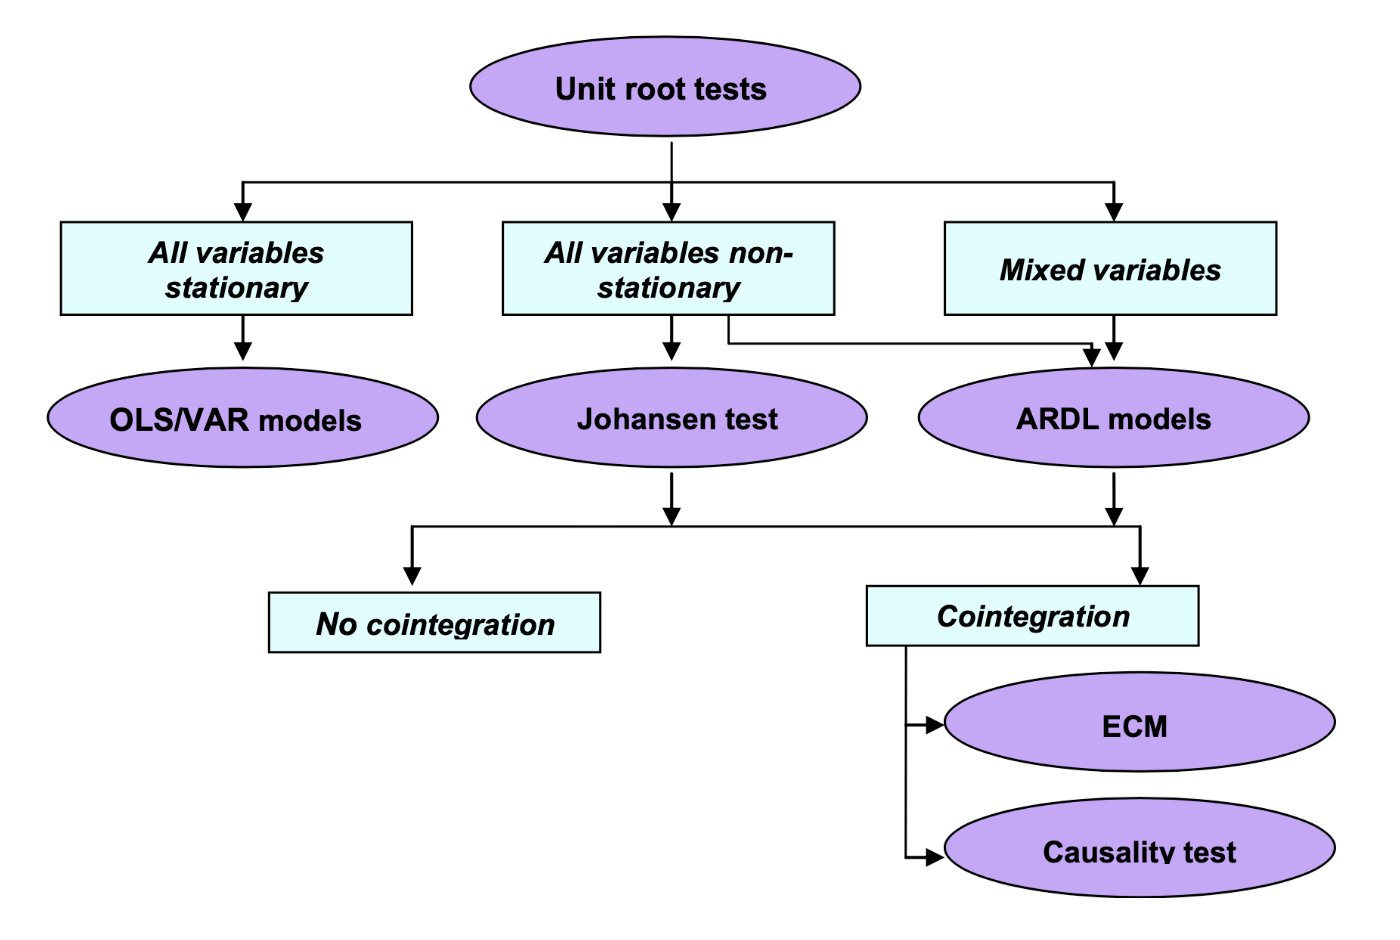
\includegraphics[width = 1.0 \textwidth]{TimeSeries_Models}
  \caption{ Method selection for time series data. OLS: Ordinary least squares; VAR: Vector autoregressive; ARDL: Autoregressive distributed lags; ECM: Error correction models, retomado de: Shrestha y Bhatta (2018) }
  \label{TimeSeries_Models}
\end{figure}

En este caso incorporaremos a los modelos autogregressive distributed
lag models (ARDL, por sus siglas en inglés). En estos casos el
procedimiento de Johansen no podría aplicarse directamennte cuando las
variables incluidas son de un orden mixto o cuando simplemente todas no
son estacionarias. Un modelo ARDL está basado en procedimientos de MCO.

Este tipo de modelos toma suficientes rezagos para capturar el mecanismo
generador de datos. También es posible llegar a una especificación del
mecanismo corrector de errores a partir de una trasformación lineal del
ARDL.

Consideremos la siguiente ecuación: \[
    Y_t = \alpha + \delta X_t + \gamma Z_t + U_t
    \label{Eq_ARDL}
\]

Dada la ecuación (\ref{Eq_ARDL}) podemos establecer su forma de
mecanismo corrector de errores en forma ARDL dada por: \begin{eqnarray*}
    \Delta Y_t & = & \alpha + \sum_{i = 1}^p \beta_i \Delta Y_{t-i} + \sum_{i = 1}^p \delta_i \Delta X_{t-i} + \sum_{i = 1}^p \gamma_i \Delta Z_{t-i} \\ 
    &  & + \lambda_1 Y_{t-1} + \lambda_2 X_{t-1} + \lambda_3 Z_{t-1} + U_t
\end{eqnarray*}

Donde los coeficientes \(\beta_i\), \(\delta_i\), \(\gamma_i\)
representan la dinámica de corto plazo y las \(\lambda\)'s la dinámica
de largo plazo.

La hipótesis nula (\(H_0\)) es que las
\(\lambda_1 + \lambda_2 + \lambda_3 = 0\), es decir, que no existe
relación de largo plazo.

En la práctica estimamos una especificación con rezafos distribuidos: \[
    Y_t = \alpha + \sum_{i = 1}^p \beta_i Y_{t-i} + \sum_{i = 1}^p \delta_i X_{t-i} + \sum_{i = 1}^p \gamma_i Z_{t-i} + U_t
\]

Además de verificar si las series involucradas son estacionarias y
decidir el número de reagos \(p\) mediante criterios de información.

\hypertarget{ejemplo}{%
\subsection{Ejemplo}\label{ejemplo}}


\printbibliography


\end{document}
